% !TEX root =  ../Report.tex

\section{Part 0: Setup your Environments}
\label{sec:Part 0} 
To begin this project, we provide 2 methods of maze generation. The first method is the simplest, and is implemented in our \texttt{createRandMaze()} function. Calling this will create a 101 X 101 boolean matrix and with a probability of 0.2, each cell is a wall. This generated numpy array is then saved once as a text file and once as a matplot figure image.

Our second method of maze generation is more sophisticated and implemented in our \texttt{createBtrackingMaze()} function. This function will use the \emph{Depth First Search} algorithm to carve a path through a boolean numpy array of all walls. After it hits a dead end, it will then backtrack its way out and create another path. The advantage of this method, is that it creates the perfect maze. Every open cell in the array can be reached by any other open cell.
\begin{figure}[H]
\begin{subfigure}{.5\textwidth}
  \centering
  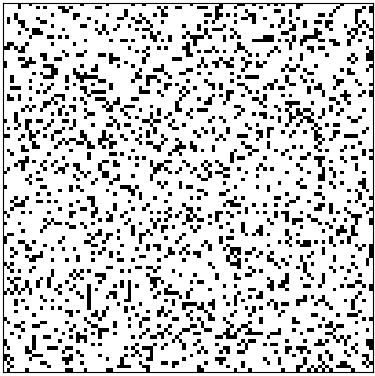
\includegraphics[width=0.8\linewidth]{Report/Part0/random.png}  
  \caption{Random maze}
\end{subfigure}
\begin{subfigure}{.5\textwidth}
  \centering
  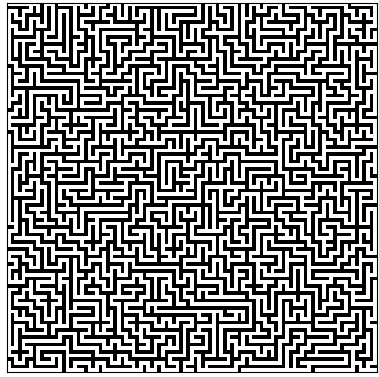
\includegraphics[width=0.8\linewidth]{Report/Part0/backtracked.png}  
  \caption{DFS backtracked maze}
\end{subfigure}
\caption{Sample maze generations}
\end{figure}

Using the above 2 methods, we will generate 25 random mazes and 25 backtracked mazes for our tests. As mentioned previously, we will also save these to file so the same mazes are used for all of our tests.